% Author: Rasmus Pank Roulund
\documentclass{minimal}
\usepackage{tikz}
\usetikzlibrary{shapes.geometric, arrows,positioning,calc,fit}

\begin{document}

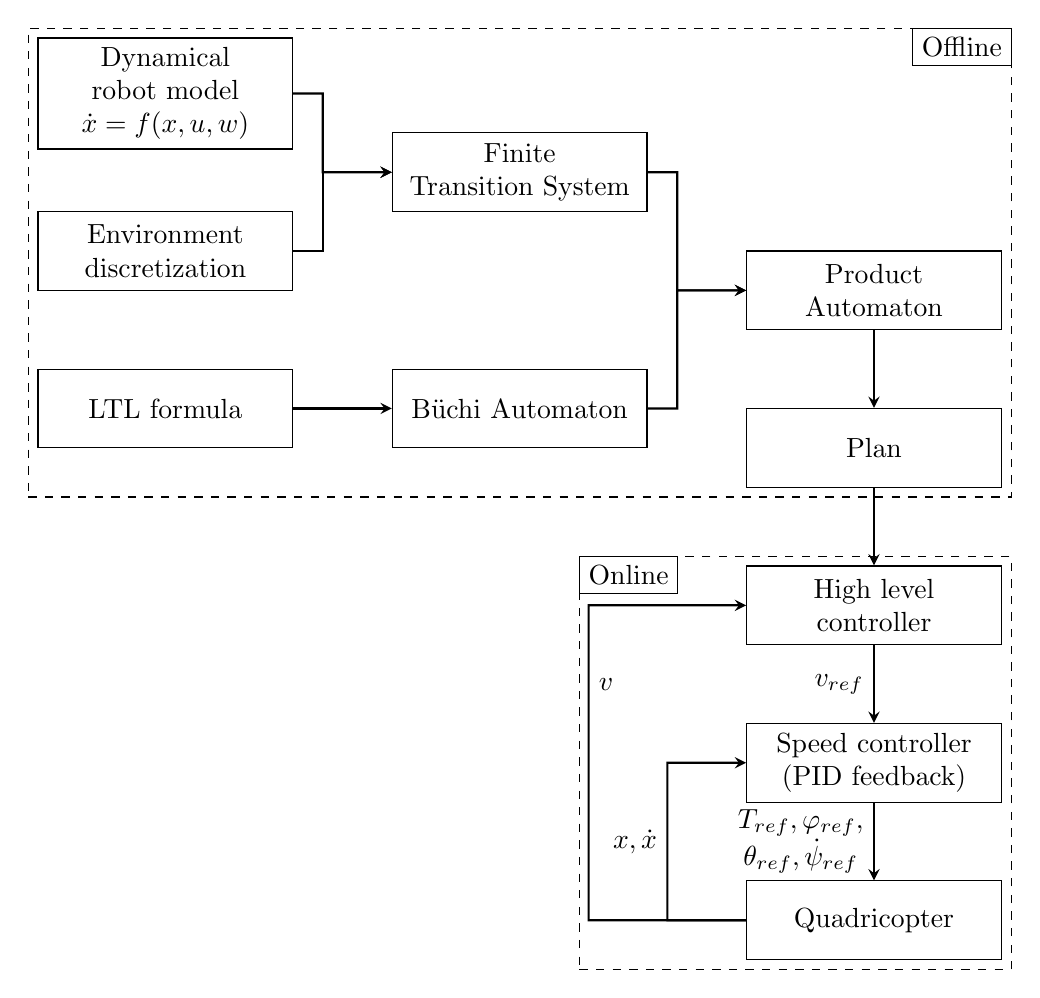
\begin{tikzpicture}[node distance = 2cm]

\tikzstyle{cell} = [rectangle, minimum width=3cm, minimum height=1cm,text centered, draw=black, text width=3cm,on grid,auto]
\tikzstyle{arrow} = [thick,->,>=stealth]

%% ------------------
%% -- OFFLINE PART --
%% ------------------

% FTS
\node (dyn_robot) 	[cell] {Dynamical robot model ${\dot{x} = f(x,u,w)}$};
\node (env) 			[cell, below of=dyn_robot] {Environment\\ discretization};
\node (fts) [cell, right of=env, xshift=2.5cm, yshift=1cm] {Finite \\Transition System};

% LTL
\node (ltl) [cell, below of=env] {LTL formula};
\node (buchi) [cell, right of=ltl, xshift=2.5cm] {B\"uchi Automaton};

% PRODUCT
\node (product) [cell, right of=fts, xshift=2.5cm, yshift=-1.5cm] {Product \\Automaton};

\node (plan) [cell, below of=product] {Plan};

\draw [arrow] (env) -- ++(2,0) -- ++(0,1.) -- (fts);
\draw [arrow] (dyn_robot) -- ++(2,0) -- ++(0,-1.) -- (fts);

\draw [arrow] (ltl) -- (buchi);

\draw [arrow] (buchi) -- ++(2,0) -- ++(0,1.5) -- (product);
\draw [arrow] (fts) -- ++(2,0) -- ++(0,-1.5) -- (product);

\draw [arrow] (product) -- (plan);

\coordinate (offline_box_pt1) at ($(dyn_robot.north west)$);
\coordinate (offline_box_pt2) at ($(plan.south east)$);

% OFFLINE BOX
\node (offline_box) [draw,dashed] [fit = (offline_box_pt1) (offline_box_pt2)] {};

\node [draw,below left] at (offline_box.north east) {Offline};

%% -----------------
%% -- ONLINE PART --
%% -----------------

\node (controller) [cell, below of=plan] {High level \\controller};
\draw [arrow] (plan) -- (controller);

\node (speed_controller) [cell, below of=controller] {Speed controller\\ (PID feedback)};
\draw [arrow] (controller) -- (speed_controller) node[pos=0.5, anchor=east] {$v_{ref}$};

\node (quad) [cell, below of=speed_controller] {Quadricopter};
\draw [arrow] (speed_controller) -- (quad) node[align=center,pos=0.5, anchor=east] {$T_{ref},\varphi_{ref},$ \\$\theta_{ref},\dot{\psi}_{ref}$};

\draw [arrow] (quad.west) -- ++(-1,0) -- ++(0,2) node[align=center,pos=0.5, anchor=east] {$x,\dot{x}$} -- (speed_controller);

\draw [arrow] (quad.west) -- ++(-2,0)  -- ++(0,4) node[align=center,pos=0.75, anchor=west] {$v$} -- (controller);


\coordinate (online_box_pt1) at ($(controller.north west) - (2,0)$);
\coordinate (online_box_pt2) at ($(quad.south east)$);

% ONLINE BOX
\node (online_box) [draw,dashed] [fit = (online_box_pt1) (online_box_pt2)] {};

\node [draw,below right] at (online_box.north west) {Online};



\end{tikzpicture}

\end{document}
